\chapter{First-hitting-time models}

\section{Survival data and basic definitions}
Survival analysis is the field of studying lifetime and time-to-death data. 

\subsection{General idea}
Consider studying the time to an event of interest. You might be a doctor performing a study of cancer patients, and monitoring them
for possible relapse. In this case, the event is the relapse. Or, possibly, you are a demographer looking at all parents who have only one child, and you are monitoring the time that elapses before they have a second child.
While these events are a relapse and a birth, respectively, we will
collectively refer to them as deaths, and hence the time to the event happens we call time-to-death.
The time-to-death $T$ is a stochastic variable and of a non-negative domain.
Clearly, to observe such data in real life, we must wait until the event actually happens. This might in some cases never happen, or it might take a very long time. Consider a clinical trial of $n$ patients who have been treated for some disease, and where $T_i$, $i=1,\ldots,n$, is the time until their relapse. Such a trial can only last a certain amount of time, say, until $\tau$.
Luckily, not every patient relapses during that time, and so the actual time to their relapse, $\tilde{T}_i$, is not observed. Note that it might turn out that the actual $\tilde{T}_i$ does not exist.
We could throw away these observations without an observed event. But we at least know that these patients survived until time $\tau$. We therefore work with the concept of incomplete data, which we call \textit{censored} data.

An overview of modelling survival data is \citet{ABG}.

\subsection{Independently censored survival data}
An observed lifetime $T$ is censored if the actual lifetime $\tilde{T}$ is larger than $T$. We can say that we have a censoring mechanism which works such that the observed $T$ is $T=\min(\tilde{T}, C)$, where $C$ is a certain censoring time. In the clinical trial example mentioned, the censoring time $C$ would be the end of the possible observation period of the trial, namely $\tau$.
To go with the censoring mechanism, we need a censoring indicator, which we denote $d$. It is defined as
\begin{equation}\label{eq:censoring}
    d=\indicator(T=\tilde{T}),
\end{equation}
indicating if we have observed the actual event. If the event has occurred, the indicator $d$ is 1, and if not, it is 0. An important definition is the concept of \textit{independent censoring}. We say that we have independent censoring if the censoring indicator $d$ is independent of the time, meaning that
\begin{equation*}
    P(t|d)=P(t).
\end{equation*}
An example where we do not have independent censoring is ...

\subsection{The survival function $S(t)$, the hazard function $\hz(t)$, and their estimators}
In survival analysis, one of the things we are interested in is the survival function. The survival function $S(t)$ is the probability of surviving until time $t$,
\begin{align*}
    S(t)=\Pr(T>t)=1-\Pr(T<t)=1-F(t).
\end{align*}
Here $F(t)$ is the familiar cumulative distribution function. If $F(t)$ is the cumulative distribution has a derivative $f(t)$ which exists, then the lifetime $T$ has probability distribution function (pdf) $f(t)$.

We are also interested in the hazard function. This is the probability of the event happening at time $t$, conditioned on the event not having happened yet. More formally, the hazard function is defined as
\begin{equation*}
    \hz(t)=\lim_{\epsilon\to0}\frac{\Pr(T<t+\epsilon|T>t)}{\epsilon}.
\end{equation*}
Estimating the hazard function is hard, and we do not achieve the usual $\sqrt{n}$ convergence.
\todo[inline]{add citation}
It is, however, typically the function we are most interested in, as we will see later, in subsection \ref{subsec:ph-reg}.
Note that by observing
\begin{equation*}
    \Pr(T<t+\epsilon|T>t)=\frac{\Pr(T<t+\epsilon,T>t)}{\Pr(T>t)}=\frac{F(t+\epsilon)-F(t)}{S(t)},
\end{equation*}
and inserting this into the hazard function we have the relation
\begin{equation}
\label{eq:hfs}
    \hz(t)=\frac{1}{S(t)}\lim_{\epsilon\to0}\frac{F(t+\epsilon)-F(t)}{\epsilon}=\frac{f(t)}{S(t)}=\frac{-S^\prime(t)}{S(t)},
\end{equation}
where the probability distribution function $f(t)$ is obtained by its limit definition, and we note that $S^\prime(t)$ is the derivative of $1-F(t)$, which is $-f(t)$. We further note that by interchanging the notation for derivation, we obtain
\begin{equation}\label{eq:alpha-diff}
\alpha(t)=\frac{S^{\prime}(t)}{S(t)}=\frac{\frac{\d S}{\d t}}{S(t)}.
\end{equation}
By integrating the hazard from 0 to time $t$, we get the cumulative hazard function,
\begin{equation}\label{eq:cumulative-hazard-1}
    A(t)=\int_0^t\hz(s)\d s,
\end{equation}
and we insert \eqref{eq:alpha-diff} into \eqref{eq:cumulative-hazard-1},
\begin{equation}\label{eq:cumulative-hazard}
\begin{split}
     A(t)=-\int_0^t\frac{\frac{\d S}{\d s}}{S(s)}\d s=-\int_0^t\frac{1}{S(s)}\d S=-\log(S(t)),
\end{split}
\end{equation}
which is an important relationship.
Given survival data $(t_i,d_i)_{i=1}^n$, we introduce the \textit{risk set} $R(t)$, which gives the set of all individuals at risk at time $t$,
\begin{equation*}
    R(t)=\{t\colon t_i\geq t\}.
\end{equation*}
We further introduce the function $Y(t)$, which is equal to the number of individuals still at risk at time $t$,
\begin{equation*}
    Y(t)=\#R(t)=\#\{t\colon t_i\geq t\},
\end{equation*}
where $\#(\cdot)$ is the counting operator over a set. Note that $Y(t)$ does not depend on the censoring indicators, since
an individual is at risk at time $t$ even though it turns out that it did not die, i.e., its censoring indicator $d_i$ is 0.
Estimating the survival function $S(t)$ is done by the Kaplan-Meier estimator \citep{kaplan-meier},
\begin{equation*}
    \hat{S}(t)=\prod_{i:\{t_i\leq t\}}1-\frac{d_i}{Y(t_i)},
\end{equation*}
and the cumulative hazard function $A(t)$ by the Nelson-Aalen estimator \citep{nelson, aalen1978},
\begin{equation*}
    \hat{A}(t)=\sum_{i:\{t_i\leq t\}}\frac{d_i}{Y(t_i)}.
\end{equation*}

\section{Classical inference approaches}
\subsection{Likelihood regression}
Consider survival data $(t_i,d_i),\,i=1,2,\ldots,N$, where $t_i$ is the time to death of individual $i$, and $d_i$ is a censoring indicator of the usual type, meaning it is 1 if the death has been observed, and 0 if not.
To make inference on what affects the time to death, we need to consider covariates. Covariates are information about an individual. In medical applications, typical covariates are age, gender, disease status, as well as clinical measurements.
Denote the covariates, i.e., the information, of an individual $i$ by $x_{i,1},x_{i,2},\ldots,x_{i,p}$, where $p$ is the number of pieces of information. We gather these in a vector $\x_i=(x_{i,1},x_{i,2},\ldots,x_{i,p})$. We may now consider a data set of complete tuples of survival data with covariates,
\begin{equation}\label{eq:surv-D}
    D=(t_i,d_i,\x_i)_{i=1}^N.
\end{equation}
Now, consider a survival time distribution $\psi(\bbeta)$, which has a vector of regression parameters $\bbeta=(\beta_1,\beta_2,\ldots,\beta_p)$, with one parameter $\beta_j,\,j=1,2,\ldots,p$ corresponding to one covariate $x_j$. This distribution has a parameterized survival function
\begin{equation*}
    S(t|\bbeta,\x)
\end{equation*}
and a parameterized probability distribution function
\begin{equation*}
    f(t|\bbeta,\x).
\end{equation*}
Given an observed dataset $D$ \eqref{eq:surv-D}, we wish to make inference on which covariates affect the survival time. One way to do this, having assumed a specific survival distribution $\psi(\bbeta)$, is to construct a so-called (joint) likelihood.
The likelihood is an expression for the probability of observing the observed sample, as a function of the parameters $\bbeta$ in the distribution. If all censoring indicators are 1, meaning all observations are actual deaths,
we are in the usual statistical regression landscape. For each observation, its likelihood is the probability of observing its death at $t_i$ given the parameters and the data,
\begin{equation*}
    f(t_i|\bbeta,\x_i).
\end{equation*}
A typical assumption when setting up a (joint) likelihood is to assume that the conditional distribution of each observation is independent and identically distributed (\textit{iid}), given the data. Hence the joint likelihood is the product of all the single likelihood contributions,
\begin{equation}
    L(\bbeta)=\prod_{i=1}^N f(t_i|\bbeta,x_i).
\end{equation}
But we need to consider the case of censored survival data, and we wish to set up a joint likelihood for such a data set.
Again assume that the data $D=\{x_i,y_i\}_{i=1}^n$ is independent and identically distributed from a survival distribution $\psi(\bbeta)$.
In the case of an uncensored observation $i$, meaning $d_i=1$, it contributes
\begin{equation}\label{eq:f}
    f(t_i|\bbeta,\xi)
\end{equation}
to the likelihood. If the event has not occurred, the observation is censored, and $d_i$ is 0. In this case, we do not have the actual lifetime, and so we cannot use the lifetime distribution, but we must instead use the survival distribution.
After all, the fact that this individual is alive at time $t_i$ is informative.
Therefore this observation contributes
\begin{equation}\label{eq:S}
    S(t_i|\bbeta,\xi)
\end{equation}
to the likelihood. Since an observation can only be either censored or not censored at the same time, $d_i$ is either 0 or 1. This means that we can combine expressions \eqref{eq:f} and \eqref{eq:S} in a way that a single observation contributes the product
\begin{equation*}
    f(\ti|\x_i)^{d_i}S(\ti|\x_i)^{1-d_i}
\end{equation*}
to the likelihood. Since we assume the observations to be independent, the likelihood is, again, the product of the single complete contributions. The complete likelihood becomes
\begin{equation}\label{eq:surv-lik}
    L(\bbeta)=\prod_{i=1}^n f(t_i|\x_i,\bbeta)^{d_i} S(t_i|\x_i,\bbeta)^{1-d_i}.
\end{equation}
It is more convenient to work with the log likelihood,
\begin{align}\label{eq:surv-log-lik}
\begin{split}
    l(\bbeta)&=\log L(\bbeta) \\
    &=\sum_{i=1}^n\left[ d_i \log f(t_i|\x_i,\bbeta) + (1-d_i)\log S(t_i|\x_i,\bbeta)\right].
\end{split}
\end{align}
Note that since $A(t)=-\log S(t)$ and $f(t)=\alpha(t)S(t)$, see \eqref{eq:cumulative-hazard} and \eqref{eq:hfs}, respectively, \eqref{eq:surv-log-lik} further simplifies to
\begin{equation*}
    l(\bbeta)=\sum_{i=1}^n\left[ d_i \log \hz(t_i|\x_i,\bbeta) - A(t_i|\x_i,\bbeta)\right].
\end{equation*}

\subsection{Proportional hazards regression}\label{subsec:ph-reg}
In other fields of statistics, we are often most interested in modelling the probability distribution function
and the cumulative distribution function.
In survival analysis, however, we are typically more interested in modelling the hazard function. The reasons for this will become clear in a minute.

In this subsection, we consider the effect of covariates on the hazard function $\hz(\cdot)$. How may we use a covariate vector $\x$ in modelling the hazard rate? A very common model to choose here is that of a proportional hazards model, which assumes
\begin{equation}\label{eq:PH}
    \hz(t|\x)=\hz_0(t)r(\x|\bbeta),
\end{equation}
where $\hz_0(t)$ is an \textit{unspecified} baseline hazard function shared between all individuals, and $r(\x|\beta)$ is a so-called relative risk function parameterized with regression coefficients $\bbeta=(\beta_1,\ldots,\beta_p)$. We choose $r(\x)$ such that it is appropriately normalized, meaning $r(\0)=1$.
A crucial assumption here is that the effects of the covariates are fixed in time. In this setup, it turns out that we can do regression without specifying the baseline hazard. This is a major advantage, because we then do not have to think about modelling effects in time. Given data $D=(t_i,d_i),i=1,\ldots,n$, we may set up a so-called partial likelihood.

The idea behind the partial likelihood is as follows. Since we have observed data $D$ with at least some censoring indicators $d_i$ equal to 1. In partial likelihood regression, we simply ignore the censored observations.
Informally, the probability of the event happening at a time $t$ for some individual $j$ is the probability of an event happening to individual $i$ at
time $t$, divided by the total probability of an event happening at time $t$,
the instantaneous probability of an event happening to that individual at that time, i.e., the hazard function of that individual at that time,
\begin{equation}\label{eq:hazard-frac-informal}
    \frac{\Pr(\text{event happens to individual }i\text{ at time }t)}{\Pr(\text{event happens to any individual }j\text{ at time }t)}.
\end{equation}
More formally, we look at the instantaneous probability of an event happening for the individual $i$, which is the hazard function $\hz(t|\x_i)$.
Thus the total probability of an event happening at time $t$ is the sum of the hazard functions of all individuals in the risk set
$R(t)$, which, again, is defined as
\begin{equation*}
    R(t)=\{i\colon t_i\geq t\,,i=1,2,\ldots,n\}.
\end{equation*}
From all the uncensored observations, we know that events happened at times $\{t_i\colon d_i=1,\,i=1,2,\ldots,n\}$. Therefore, we can construct expressions for \eqref{eq:hazard-frac-informal} at all the observed, uncensored, times.
Inserting the probabilities into the informal expression in \eqref{eq:hazard-frac-informal}, an individual with an observed death at $t_i$ 
contribues to the likelihood with
\begin{equation}\label{eq:hazard-frac}
    \frac{\hz_0(t_i)r(\x_i)}{\sum_{j\in R(t_i)} \hz_0(t_i)r(\x_j)}.
\end{equation}
Now, assuming that observations are independent and identically distributed, we say that the \textit{partial likelihood} of the model
given the observed data is the product of all ratios \eqref{eq:hazard-frac}, is
\begin{equation}\label{eq:pl}
    \pl(\bbeta)=\prod_{i\colon d_i=1}\frac{\hz_0(t_i)r(\x_i)}{\sum_{j\in R(t_i)} \hz_0(t_i)r(\x_j)},
\end{equation}
The baseline hazard will cancel out in expression \eqref{eq:pl}, and we are left with just the relative risk functions,
\begin{equation*}
    \pl(\bbeta)=\prod_{i\colon d_i=1}\frac{r(\x_i)}{\sum_{j\in R(t_i)}r(\x_j)}.
\end{equation*}
The fact that the baseline hazard cancels out is quite powerful. Even though proportional hazards regression is not fully parametric,
the canceling means that we can fully model the effect of covariates without having to consider the baseline hazard.

We have not said anything about what $r(\x)$ looks like. The most common choice, by far, for $r(\x)$ is
\begin{equation*}
    r(\x)=\exp(\x^T\bbeta),
\end{equation*}
which leads to the famous Cox model \citep{cox1965}. The Cox model is an attractive model because the effect of a unit increase in an element of $\bbeta$ has a nice interpretation. Assume we have two observations with covariate vectors $\x_1$ and $\x_2$, and that $\x_2$ is equal to $\x_1$ except for in element $j$, where $x_{2j}=x_{1j}+1$. Then the ratio of the two hazard rates becomes
\begin{equation*}
    \frac{\exp(\x_2^T\bbeta)}{\exp(\x_1^T\bbeta)}=\exp((\x_2-\x_1)^T\bbeta)=\exp(\beta_j).
\end{equation*}
Furthermore, if the two covariate vectors differ in more elements, say, that, each element in $\x_2$ is one unit increased from each element in $\x_1$, we get that
\begin{equation*}
    \frac{\exp(\x_2^T\bbeta)}{\exp(\x_1^T\bbeta)}=\exp((\x_2-\x_1)^T\bbeta)=\exp(\beta_1+\beta_2+\ldots+\beta_p)=\exp(\beta_1)\exp(\beta_2)\cdots\exp(\beta_p).
\end{equation*}
In other words, each unit increase in a covariate is a multiplicative factor in the hazard. Cox regression is used very much in applied research. We will here give a simple example to illustrate its use.

\subsection{Cox regression example}
Lorem ipsum.

\subsection{Issues with the proportional hazards assumption}
Assuming \eqref{eq:PH}, i.e. $\hz(t|\x)=\hz_0(t)r(x|\bbeta)$, we are making a relatively strong assumption. Namely, we assume that the ratio between the hazard function of two individuals is the same \textit{at all times}, because the part of $\hz(t|\x)$ cancels out when we do regression, and because we assume that the covariate effects are constant in time, as $r(x|\bbeta)$ is not a function of time.
This assumption goes under the name of the proportional hazards (PH) assumption. While, as we saw, this assumption greatly simplifies the inference, it is not necessarily satisfied in practice. In any case, it is very difficult to verify. There exist alternative models, which do not assume the PH assumption. One of these is Aalen's additive model, which is an example of additive hazard modelling. In Aalen's model, the hazard function takes the form
\begin{equation}
    \alpha(t|\x)=\beta_0(t)+\beta_1(t)x_1(t)+\beta_2(t)x_2(t)+\ldots+\beta_p(t)x_p(t),
\end{equation}
where $\beta_j(t),j=1,\ldots,p$ is the increase in the hazard at time $t$ corresponding to a unit's increase in the $j$-th covariate. Another alternative model to the Cox model is the first hitting threshold model. In this thesis we will focus on this model, which has not seen methods developed for it so as to be able to use it in typical clinical settings for biomedical data, such as on gene expression data.

\subsection{Robustness of Cox when the PH assumption is violated}
Although the PH assumption is often not valid, in practice, Cox regression tends to work well. \todo[inline]{Need to find a citation here.}

\subsection{Cox, proportional hazards, and variable selection}

\section{First hitting time models}\label{sec:FHT}
So far we have done regression by modelling the hazard rate $\hz(\cdot)$.
Therefore we have not thought much about how a time-to-death is \textit{generated}, other than the fact that it arises from a survival distribution $S(\cdot)$ with a corresponding hazard function $\hz(\cdot)$.
In this context, an individual is alive at one time. Slightly later, it is either still alive, or it may have died.
One way to think about how these times are generated, without thinking about probability distributions just yet, is to imagine that each 
individual has an underlying stochastic process, a health process $Y(t)$, say. When this health process reaches some barrier, or some end state, the individual dies. This is a conceptual appealing framework, because, instead of just a stochastic lifetime, it introduces
the concept of distance to death. We may call the time the health process hits this barrier or end state for the \textit{first hitting time} (FHT)
of a boundary or threshold state, by sample paths of a stochastic health process. This health process may be latent, i.e., unobservable,
or it may be observable.
Many types of time-to-death data may, in fact, be interpreted as FHTs.
FHT models have a long history of application in diverse fields, including medicine and engineering. FHT models have been used to describe the length of a hospital stay \citep{whitmore1975,eaton-whitmore}, and to model the duration of a strike \citep{lancaster}. They have also been used to estimate degradation in components \citep{whitmore1995}, and to assess lung cancer risk in railroad workers \citep{leewhitmore2004}.

\subsection{General idea}\label{fht-idea}
A first-hitting-time (FHT) model has two basic components:
\begin{enumerate}
\item A parent stochastic process $\{Y(t),\,t\in\setT,\,y\in\setY\}$, with initial value $Y(0)=y_0$, where $\setT$ is the time space and $\setY$ is the state space of the process.
\item A boundary set $\setB$, where $\setB\subset\setY$. This is at times also referred to as a barrier or a threshold, depending on which is most appropriate to the context.
\end{enumerate}
The process $\{Y(t)\}$ may have a variety of properties, such as one or many dimensions, the Markov property, continuous or discrete paths, and monotonic sample paths. Whether the sample path of the parent process is observable or latent (unobservable) is an important distinguishing characteristic of the FHT model. Latent (unobservable) processes are the most common by far. The boundary set $\setB$ may also have different features. The basic model assumes that $\setB$ is fixed in time. In some applications, however, it varies with time, i.e., $\setB(t)$. This is, however, out of the scope of this thesis.

Taking the initial value $Y(0)=y_0$ of the process to lie outside the boundary set $\setB$, the \textit{first hitting time} of $\setB$ is the random variable $S$ defined as
\begin{equation}\label{eq:fht-t}
    T=\inf_t\left(t\colon Y(t)\in\setB\right).
\end{equation}
Thus, the first hitting time is the time when the stochastic process first encounters the boundary set $\setB$. The boundary set defines a stopping condition for the process. Note that when the parent process is latent, there is no direct way of observing the FHT even in the state space of the process.

In some versions of the FHT model, there is no guarantee that the process $\{Y(t)\}$ will reach the boundary set $\setB$, so $P(T<\infty)<1$. We will let $T=\infty$ denote the absence of a finite hitting time with
\begin{equation}
    P(T=\infty)=1-P(T<\infty).
\end{equation}
This condition is sometimes plausible and a desirable model feature.
Two common concepts in survival analysis might lead to this.
One is the case of competing risks.
That is the case where an individual might die from not only one, but several causes, but we are only studying one of these.
Naturally, then, we would not except that all individuals die from the cause that we study, and hence $P(T<\infty)<1$.
The second concept is what models that aee often called ``cure models'', or, models with ``long-term survivors.''
A cure model is a model where there are individuals with zero frailty, i.e., a nonsusceptible group \citep{ABG}.
Consult \citet{maller1996survival} for a book on this.

\citet{eaton-whitmore} discuss FHTs as a general model for hospital stay. \citet{aalengjessing2001} provide an overview of much of this subject. \citet{lawless2011} provides a compact overview of the theory. \citet{leewhitmore2004a} provides an overview of first hitting time models for survival and time-to-event data. There is a large literature dealing with theoretical and mathematical aspects of FHT models.

Models based on this view are called first hitting time models (FHT). FHT models were introduced in \citet{whitmore1986}, see \citet{leewhitmore2006} for a complete overview. Note that these authors use the term threshold regression when referring to regression for first hitting time models. We have, following \citet{caroni2017}, chosen to not use this term, as it is already referring to a well established, and quite different, topic in econometrics. First-hitting-time models have been applied to many different fields, including medicine, engineering, and economics, and used, for example to describe the survival time of a transplant patient\todo{citation needed}, the duration time of a strike \citep{lancaster}, the failure time of an engineering system \todo{citation needed}, and so on.

\subsection{Examples of first-hitting-time models}
The parent stochastic process may take many forms, from Wiener processes to Markov chains. Similarly, the boundary state may take various forms. For example, it may be a fixed threshold in a Wiener process or an absorbing state in a Markov chain. This choice in process and boundary shows that the FHT framework is highly flexible. The choice of boundary must fit the process, such that the boundary set is a subset of the state space.
\begin{enumerate}
    \item \textit{Bernoulli process and negative binomial first hitting time.}The number of trials $S$ required to reach the $m$-th success in a Bernoulli process $\{B_t,t=1,2,\ldots\}$ has a negative binomial distribution with parameters $m$ and $p$, where $p$ is the success probability of each trial. To give this setup our standard representation, we consider a parent process
    \begin{equation*}
        \{Y(t),\,t=0,1,2,\ldots\}
    \end{equation*}
    with initial value $Y_0=y_0=m$ and let
    \begin{equation*}
        Y_t=y_0-B_t,\,t=1,2,\ldots,
    \end{equation*}
    where $\{B_t\}$ is the aforementioned Bernoulli process. The first hitting time is the first Bernoulli trial $t=T$ for which $Y_t$ equals 0. The number of rocket launches to get $m$ satellites in orbit is an example of this FHT model.
    \item \textit{Gamma process and inverse gamma first hitting time.} Consider a parent process
    \begin{equation*}
        \{Y(t),\,t\leq0\}
    \end{equation*}
    with initial value $Y(0)=y_0>0$. Let
    \begin{equation*}
        Y(t)=y_0-Z(t),
    \end{equation*}
    where $Z(t),\,t\leq0$ is a gamma process with a scale parameter $\beta$, a shape parameter $\alpha$ and a starting point $Z(0)=0$. The first hitting time of the zero level in the parent process ($Y=0$) has an inverse gamma cumulative distribution function (cdf), defined by the identity
    \begin{equation}
        P(T>t)=P(Z(t)<y_0).
    \end{equation}
    The identity follows from the fact that a gamma process has monotonic, nondecreasing sample paths. Computational routines for the gamma cdf allows the cdf of T to be computed readily. \citet{singpurwalla1995} and \citet{lawless2004} consider the gamma process as a model for degradation.
\end{enumerate}
If we consider the health process to be analogous with a person's health, this makes sense. A person's health, although generally decreasing over longer periods of time, will fluctuate, at times going up, and at times going down. If we do, however, want a monotonic restriction on the movement of the health process, we may use a gamma process \citep{leewhitmore2006}. This might make sense if the health process is meant to model e.g. the breakdown of a structure. Another usual setup for a first hitting time model is to have the health process be a Wiener process, and the boundary set be a fixed threshold level. This is attractive because it has closed-form probability and cumulative density functions, and its likelihood is computationally simple. There are also no restrictions on the movements of the process, meaning, it is non-monotonic. We will first give an introduction to the Wiener process.

\subsection{Wiener process}
Consider a continuous stochastic process $W(t)$ defined for $t\in[0,\infty)$, taking values in $\R$, and with initial value $W(0)=0$. If $W$ has increments that are independent and normally distributed with
\begin{equation*}
    \E[W(s+t)-W(t)]=0\text{   and   }\Var[W(s+t)-W(t)]=s,
\end{equation*}
we call $W$ a Wiener process. In other words, each increment has expectation 0 and has standard deviation proportional to the length of the time interval. The position of the process at time $t$ always follows a Gaussian distribution $N(0, t)$ \citep{ABG}. To increase the flexibility of the Wiener process, we can introduce a new process $Y$,
\begin{equation}\label{wiener}
    Y(t)=y_0-\mu t+\sigma W(t),
\end{equation}
which is called a Wiener process with initial value $y_0$, drift coefficient $\mu$, and diffusion coefficient $\sigma$. A good introduction to Wiener processes can be found in \citet{cox1965}.
\begin{figure}[H]
\label{plot:wiener}
\caption{Example of 5 Wiener process paths with initial value $y_0=10$ and drift $\mu=1$.}
\centering
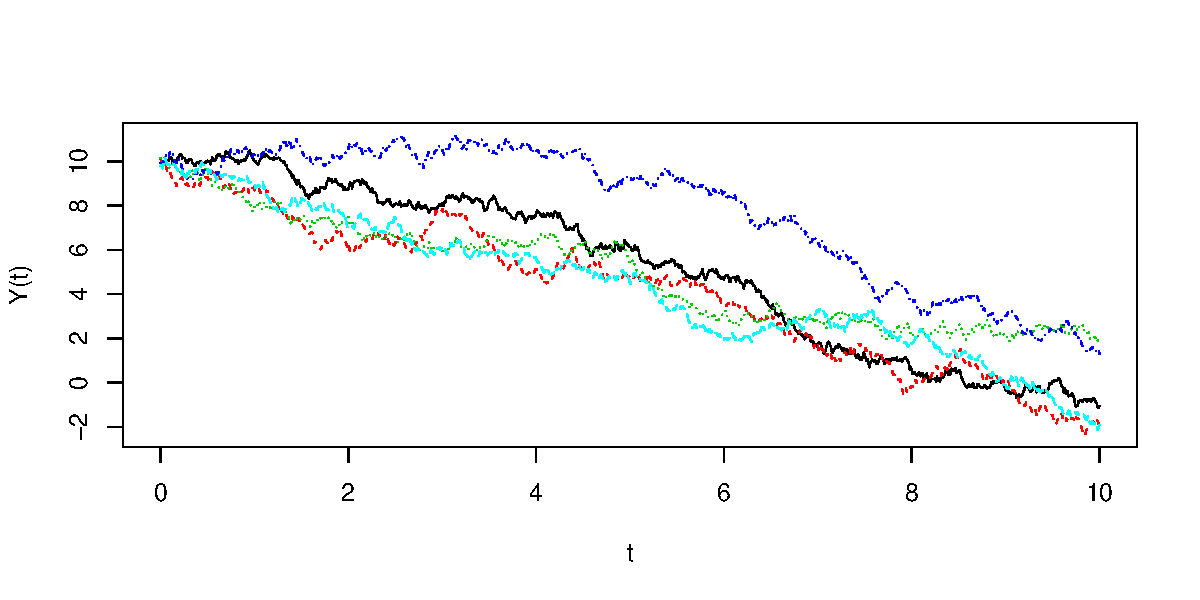
\includegraphics[scale=0.4]{figures/wiener_processes.pdf}
\end{figure}
\noindent{}Clearly, for a Wiener process starting in $y_0>0$ and with a downwards drift, i.e. $\mu>0$, the movement is markedly in the direction of zero. If $\sigma^2$ is small in comparison to the drift, as well as that the initial level is sufficiently high in comparison to $\sigma^2$, then the process will move in almost a straight line, such that
\begin{equation*}
    X(t)\approx y_0-\mu t.
\end{equation*}
Consequently, the first hitting time will be nearly a deterministic function of $y_0$ and $\mu$,
\begin{equation}
    T\approx \frac{y_0}{\mu}.
\end{equation}
This is quite visible in Figure \ref{plot:wiener}, which shows examples of 5 Wiener process paths with initial value $y_0=10$ and drift $\mu=1$. If $\sigma^2$ is relatively large compared to the drift, the diffusion part is more dominant and thus the hitting time is less predictable \citep{ABG}.

\subsection{Inverse Gaussian distribution and different parameterizations}


\subsection{Wiener process and Inverse Gaussian first hitting time}
If we choose the stochastic process to be a Wiener process like in \eqref{wiener}, and we let the boundary be the non-positive numbers, $\setB=(-\infty,0]$, then \eqref{eq:fht-t} becomes
\begin{equation}
    T=\min_t\left(t\colon Y(t)\in\setB\right),
\end{equation}
i.e. the first hitting time is the time it takes for the process to first reach a non-positive value.
(Note that since the Wiener process is continuous, there is no difference between $\leq$ and $<$. We therefore use $<$ for convenience.)
It can be shown that the first hitting time of the Wiener process follows an inverse Gaussian distribution \citep{chhikara1988}, with probability distribution function (pdf)
\begin{equation}
\label{eq:ig-pdf}
    f(t|y_0,\mu,\sigma^2)=\frac{y_0}{\sqrt{2\pi\sigma^2t^3}}\exp\left[-\frac{(y_0+\mu t)^2}{2\sigma^2t}\right],
\end{equation}
and cumulative distribution function (cdf)
\begin{equation}
\label{eq:ig-cdf}
    F(t|\mu,\sigma^2,y_0)=\Phi\sqb*{-\frac{\mu t+y_0}{\sqrt{\sigma^2t}}}+\exp\p*{-\frac{2y_0\mu}{\sigma^2}}\Phi\sqb*{\frac{\mu t-y_0}{\sqrt{\sigma^2t}}}.
\end{equation}
As previously discussed in subsection \ref{fht-idea}, note that if the drift $\mu$ is positive, then it is not certain that the process will ever reach 0. Hence the probability distribution function in \eqref{eq:ig-pdf} is improper. In this case, the probability of the time not being finite is
\begin{equation}\label{eq:P-inf-FHT}
    \Pr{(T=\infty)}=1-\Pr{(T<\infty)}=1-\exp{(-2y_0\mu)},
\end{equation}
see \citet{cox1965}. Since we in survival analysis prefer working with the survival function $S(t)=1-F(t)$ rather than the cdf $F(t)$, we note that $S(t)$ becomes
\begin{equation}
\label{eq:ig-surv}
    S(t|\mu,\sigma^2,y_0)=\Phi\sqb*{\frac{\mu t+y_0}{\sqrt{\sigma^2t}}}-\exp\p*{-\frac{2y_0\mu}{\sigma^2}}\Phi\sqb*{\frac{\mu t-y_0}{\sqrt{\sigma^2t}}},
\end{equation}
where $\Phi(x)$ is the cumulative distribution function of the standard normal,
\begin{equation*}
    \Phi(x)=\int_{-\infty}^x\phi(y)\dy,
\end{equation*}
where $\phi(x)$ is the pdf of the standard normal, defined as
\begin{equation}
    \phi(x)=\frac{\exp\left(-x^2/2\right)}{\sqrt{2\pi}}.
\end{equation}
Note that we in \eqref{eq:ig-surv} used the fact that the cdf of the standard normal distribution is symmetric around 0,
meaning that we were able to swap
\begin{equation*}
    1-\Phi\sqb*{-\frac{\mu t+y_0}{\sqrt{\sigma^2t}}}
\end{equation*}
for
\begin{equation*}
    \Phi\sqb*{\frac{\mu t+y_0}{\sqrt{\sigma^2t}}}.
\end{equation*}

\subsection{The inverse gaussian is overdetermined if the health process is latent}
There are three parameters in the inverse Gaussian distribution, namely $y_0, \mu$ and $\sigma$.
We observe, however, that both the pdf $f(t|y_0,\mu,\sigma^2)$ in \eqref{eq:ig-pdf} and the survival function $S(t|\mu,\sigma^2,y_0)$ in \eqref{eq:ig-surv} only depend on these parameters through the ratios $\mu/\sigma$ and $y_0/\sigma$.
Hence, there are in reality only two free parameters. In other words, we can without loss of generality fix one parameter. The conventional way to proceed is to set $\sigma$ equal to 1 \citep{leewhitmore2006}. We will use this to make inference.

\section{Properties of the IG functions}

\subsection{The shape of the hazard function in the inverse Gaussian model}
From \eqref{eq:hfs}, we know that the hazard function can be seen as
\begin{equation*}
    \hz(t)=f(t)/S(t).
\end{equation*}
The expression for this is rather unruly, but we can make some comments on its shape as it relates to different values for $y_0$ and $\mu$.
If $y_0$ is close to zero, we essentially get a decreasing hazard rate.
If $y_0$ is far from zero, however, we essentially get an increasing hazard rate.
If $y_0$ is somewhat inbetween, we get a hazard rate which first increases and then decreases \citep{ABG}.
In all three cases, the hazard has a peak.
This peak is dependent on both the initial level and the drift, of course. 
It is not as simple as the peak being at the mean lifetime, i.e., $y_0/\mu$.
Although the height of the peak will change both by changing both parameters, to simplify it a lot, $y_0$ mostly impacts at what time the
peak is, whereas $\mu$ mostly affects the height of the peak.
Regardless of the initial value, the hazard rate converges to the same limiting hazard, which is
\begin{equation}
    \lim_{t\to\infty}\hz(t)=\frac{1}{2}\left(\frac{\mu}{\sigma}\right)^2=0.5\mu^2,
\end{equation}
as seen in \citet{ABG}.
\todo[inline]{This is unclear}
\todo[inline]{Add plots of hazard rates here. see page 401 in ABG}
To get an intuitive feel for this, I have made an interactive website at \verb|vegarsti.shinyapps.io/FHT_Hazard|.

\subsection{Comparison of hazard rates}
It might be of particular interest to look at the ratio between two hazard rates. We might for example look at it when the drift $\mu$ is the same, but the initial level $y_0$ is different. Then the hazard ratio is strongly decreasing. This feature is the same phenomenon as that observed in frailty models, where the relative hazards often decline \citep{ABG}.
\todo[inline]{Explain better}
It is also of interest to do the converse, that is, look at the hazard ratio when the initial level is the same, but the drift is different. The result here is quite different. The ratio of the hazards has a ``bathtub'' shape, which levels off at a later time \citep{ABG}. Keep in mind here that levelling off means getting to proportional hazards.
We see that the FHT framework with a Wiener process is a highly flexible parametric model for survival analysis. Indeed, much more flexible than Cox regression, since the hazard ratios in Cox are all confined to be constant over time.
\todo[inline]{Add plot here as well; also here see ABG page 402}

\section{Regression}\label{subsec:IG-reg}
We may introduce effects from covariates by allowing $\mu$ and $y_0$ to depend on covariates $\x$ and $\z$. A simple and much used model
\citep{leewhitmore2006, caroni2017}
is to simply use the identity link function for the drift $\mu$, and to use the logarithm link function for the initial level $y_0$, since it must be positive in our framework,
\begin{equation}\label{eq:y0}
    \mu(\bbeta)=\bbeta^\T\x=\sum_{j=1}^p \beta_jx_j,
\end{equation}
\begin{equation}\label{eq:mu}
    y_0(\bgamma)=\exp(\bgamma^\T\z)\Rightarrow\ln y_0(\bgamma)=\bgamma^\T\z=\sum_{j=1}^d \gamma_jz_j.
\end{equation}
Here $\bbeta\in\R^p$ and $\bgamma\in\R^d$ are vectors of regression coefficients. Note that we may let $\x$ and $\z$ share none, some, or all elements. We will discuss consequences of this later.

Inserting the pdf \eqref{eq:ig-pdf} and the survival function \eqref{eq:ig-surv} into the log-likelihood \eqref{eq:surv-lik}, we get that the log-likelihood of a survival data set with the inverse gaussian FHT model, i.e.,
\begin{align}\label{eq:loglik}
\begin{split}
    l(y_0,\mu,\sigma)=\sum_{i=1}^n&d_i\p*{\ln y_0-\frac{1}{2}\ln\p*{2\pi\sigma^2\ti^3}-\frac{\p*{y_0+\mu\ti}^2}{2\sigma^2\ti}} \\
    &+
    (1-d_i)\ln\p*{\Phi\p*{\frac{\mu\ti+y_0}{\sqrt{\sigma^2\ti}}}-\exp\p*{-\frac{2y_0\mu}{\sigma^2}}\Phi\p*{\frac{\mu\ti-y_0}{\sqrt{\sigma^2\ti}}}}.
\end{split}
\end{align}

\subsection{Fitting an IG FHT model}
At the moment, the standard for fitting an inverse gaussian FHT model to survival data is to use numerical likelihood maximization \citep{caroni2017}. A few software packages for doing this exist.For \verb|R| \citep{Rlang}, the \verb|threg| package \citep{threg}. There does not exist any method to fit a \textit{regularized} model at the moment, nor to do automatic variable selection. \textbf{This is the reason for my thesis.}

\todo[inline]{Add regression example}

%\subsection{Example of application}
%Lorem ipsum some example. Just use numerical maximization.

%\subsection{Identification problems}

\subsection{Combining clinical and genetic data in the Inverse Gaussian FHT model}
Combining clinical and genetic data in biomedical survival analysis is a large and important goal.
The IG FHT model lends itself nicely to combining clinical and genetic data.
As discussed in \citet{aalengjessing2001}, an a priori
decision that e.g. the initial level of a health process is decided by genes, and that the health process drift is decided by
``lifestyle,'' would be an instance of this combining of data.